\documentclass{beamer}
\usetheme{metropolis}
\usepackage{../../resources/style}
\usepackage{colortbl}
\usetikzlibrary{matrix}

\newcommand{\beginnote}[1]{%
  \vfill
  {\footnotesize\textcolor{gray}{\textit{$\triangleright$ #1 (vezi slide-ul \emph{Resurse})}}}%
}

\title{Tablouri bidimensionale}
\subtitle{Parcurgeri $\cdot$ Împărțirea în zone $\cdot$ Simulări}
\author{Andrei Mihai Ciobanu}
\institute{Algolymp Summer School}
\date{}
\titlegraphic{
\includegraphics[width=4cm]{../../resources/algolymp-logo.png}}
\setbeamertemplate{frame footer}{Algolymp Summer School}

% ----------------------------------------------------------------
\begin{document}

\begin{frame}[shrink]
  \titlepage
\end{frame}

\begin{frame}{Cuprins}
  \tableofcontents
\end{frame}

% ================================================================
\section{Declarare și citire}

\begin{frame}{Ce este o matrice?}
  Un \textbf{tablou bidimensional} (matrice) are elementele aranjate pe \textbf{linii} și \textbf{coloane}.

  \smallskip
  Fiecare element are doi indici: $i$ (linia) și $j$ (coloana). Notăm \texttt{a[i][j]}.

  \smallskip
  \begin{center}
  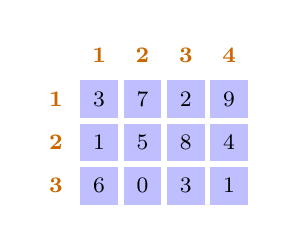
\begin{tikzpicture}
  \matrix[matrix of nodes,
          nodes in empty cells,
          ampersand replacement=\&,
          nodes={minimum size=0.48cm, text width=0.48cm, inner sep=0pt, align=center, font=\footnotesize, execute at begin node={\vphantom{0}}},
          row sep=2pt,
          column sep=2pt] {
    {} \& |[font=\footnotesize\bfseries, text=orange!80!black]| 1 \& |[font=\footnotesize\bfseries, text=orange!80!black]| 2 \& |[font=\footnotesize\bfseries, text=orange!80!black]| 3 \& |[font=\footnotesize\bfseries, text=orange!80!black]| 4 \\
    |[font=\footnotesize\bfseries, text=orange!80!black]| 1 \& |[fill=blue!25]| 3 \& |[fill=blue!25]| 7 \& |[fill=blue!25]| 2 \& |[fill=blue!25]| 9 \\
    |[font=\footnotesize\bfseries, text=orange!80!black]| 2 \& |[fill=blue!25]| 1 \& |[fill=blue!25]| 5 \& |[fill=blue!25]| 8 \& |[fill=blue!25]| 4 \\
    |[font=\footnotesize\bfseries, text=orange!80!black]| 3 \& |[fill=blue!25]| 6 \& |[fill=blue!25]| 0 \& |[fill=blue!25]| 3 \& |[fill=blue!25]| 1 \\
  };
  \end{tikzpicture}
  \end{center}

  \smallskip
  Exemplu: $n = 3$ linii, $m = 4$ coloane. \texttt{a[2][3] = 8}.
\end{frame}

\begin{frame}[fragile]{Declarare în C++}
  \begin{lstlisting}
const int NMAX = 105;
int a[NMAX][NMAX]; // declarata global
int n, m;          // dimensiunile curente
  \end{lstlisting}

  \begin{columns}[T]
    \column{0.58\textwidth}
    \begin{itemize}\itemsep2pt
      \item \textbf{Declarare globală} \textemdash{} variabilele locale stau pe \emph{stivă} ($\approx$1--8~MB); globalele în segmentul de date, mult mai mare
      \item \textbf{Convenție: indexare de la 1} \textemdash{} declarăm \texttt{a[N+1][M+1]} și lăsăm linia/coloana 0 neutilizate
      \item $1000 \times 1000$ de \texttt{int} $\approx 4$~MB \textemdash{} alegeți \texttt{NMAX} cu grijă
    \end{itemize}

    \column{0.38\textwidth}
    \begin{center}
    {\small \texttt{a[4][4]}}

    \smallskip
    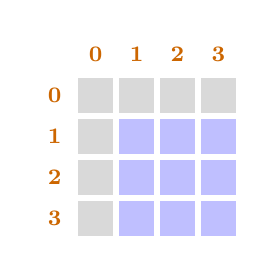
\begin{tikzpicture}
    \matrix[matrix of nodes,
            nodes in empty cells,
            ampersand replacement=\&,
            nodes={minimum size=0.45cm, text width=0.45cm, inner sep=0pt, align=center, font=\footnotesize, execute at begin node={\vphantom{0}}},
            row sep=2pt,
            column sep=2pt] {
      {} \& |[font=\footnotesize\bfseries, text=orange!80!black]| 0 \& |[font=\footnotesize\bfseries, text=orange!80!black]| 1 \& |[font=\footnotesize\bfseries, text=orange!80!black]| 2 \& |[font=\footnotesize\bfseries, text=orange!80!black]| 3 \\
      |[font=\footnotesize\bfseries, text=orange!80!black]| 0 \& |[fill=gray!30]| {} \& |[fill=gray!30]| {} \& |[fill=gray!30]| {} \& |[fill=gray!30]| {} \\
      |[font=\footnotesize\bfseries, text=orange!80!black]| 1 \& |[fill=gray!30]| {} \& |[fill=blue!25]| {} \& |[fill=blue!25]| {} \& |[fill=blue!25]| {} \\
      |[font=\footnotesize\bfseries, text=orange!80!black]| 2 \& |[fill=gray!30]| {} \& |[fill=blue!25]| {} \& |[fill=blue!25]| {} \& |[fill=blue!25]| {} \\
      |[font=\footnotesize\bfseries, text=orange!80!black]| 3 \& |[fill=gray!30]| {} \& |[fill=blue!25]| {} \& |[fill=blue!25]| {} \& |[fill=blue!25]| {} \\
    };
    \end{tikzpicture}

    \smallskip
    {\footnotesize \colorbox{gray!30}{\phantom{x}} neutilizat \quad \colorbox{blue!25}{\phantom{x}} util}
    \end{center}
  \end{columns}
\end{frame}

\begin{frame}[fragile]{Citire și afișare}
  \begin{lstlisting}
cin >> n >> m;
for (int i = 1; i <= n; i++)
    for (int j = 1; j <= m; j++)
        cin >> a[i][j];

for (int i = 1; i <= n; i++) {
    for (int j = 1; j <= m; j++)
        cout << a[i][j] << ' ';
    cout << '\n';
}
  \end{lstlisting}

  \begin{itemize}
    \item Citim mai întâi $n$ și $m$, apoi elementele \textbf{pe linii} (de sus în jos)
    \item La afișare, după fiecare linie scriem \texttt{'\textbackslash{}n'} pentru rândul următor
  \end{itemize}
\end{frame}

% ================================================================
\section{Parcurgeri}

\begin{frame}[fragile]{Parcurgere pe linii și pe coloane}
  \textbf{Pe linii} (de sus în jos):
  \begin{columns}[T]
    \column{0.64\textwidth}
    \vspace{0.47cm}
    \begin{lstlisting}[aboveskip=0pt]
for (int i = 1; i <= n; i++)
  for (int j = 1; j <= m; j++)
    // prelucreaza a[i][j]
    \end{lstlisting}

    \column{0.22\textwidth}
    \centering
    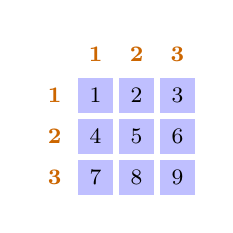
\begin{tikzpicture}
    \matrix[matrix of nodes,
            nodes in empty cells,
            ampersand replacement=\&,
            nodes={minimum size=0.45cm, text width=0.45cm, inner sep=0pt, align=center, font=\footnotesize, execute at begin node={\vphantom{0}}},
            row sep=2pt,
            column sep=2pt] {
      {} \& |[font=\footnotesize\bfseries, text=orange!80!black]| 1 \& |[font=\footnotesize\bfseries, text=orange!80!black]| 2 \& |[font=\footnotesize\bfseries, text=orange!80!black]| 3 \\
      |[font=\footnotesize\bfseries, text=orange!80!black]| 1 \& |[fill=blue!25]| 1 \& |[fill=blue!25]| 2 \& |[fill=blue!25]| 3 \\
      |[font=\footnotesize\bfseries, text=orange!80!black]| 2 \& |[fill=blue!25]| 4 \& |[fill=blue!25]| 5 \& |[fill=blue!25]| 6 \\
      |[font=\footnotesize\bfseries, text=orange!80!black]| 3 \& |[fill=blue!25]| 7 \& |[fill=blue!25]| 8 \& |[fill=blue!25]| 9 \\
    };
    \end{tikzpicture}
  \end{columns}

  \smallskip

  \textbf{Pe coloane} (de la stânga la dreapta):
  \begin{columns}[T]
    \column{0.64\textwidth}
    \vspace{0.47cm}
    \begin{lstlisting}[aboveskip=0pt]
for (int j = 1; j <= m; j++)
  for (int i = 1; i <= n; i++)
    // prelucreaza a[i][j]
    \end{lstlisting}

    \column{0.22\textwidth}
    \centering
    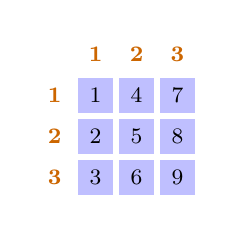
\begin{tikzpicture}
    \matrix[matrix of nodes,
            nodes in empty cells,
            ampersand replacement=\&,
            nodes={minimum size=0.45cm, text width=0.45cm, inner sep=0pt, align=center, font=\footnotesize, execute at begin node={\vphantom{0}}},
            row sep=2pt,
            column sep=2pt] {
      {} \& |[font=\footnotesize\bfseries, text=orange!80!black]| 1 \& |[font=\footnotesize\bfseries, text=orange!80!black]| 2 \& |[font=\footnotesize\bfseries, text=orange!80!black]| 3 \\
      |[font=\footnotesize\bfseries, text=orange!80!black]| 1 \& |[fill=blue!25]| 1 \& |[fill=blue!25]| 4 \& |[fill=blue!25]| 7 \\
      |[font=\footnotesize\bfseries, text=orange!80!black]| 2 \& |[fill=blue!25]| 2 \& |[fill=blue!25]| 5 \& |[fill=blue!25]| 8 \\
      |[font=\footnotesize\bfseries, text=orange!80!black]| 3 \& |[fill=blue!25]| 3 \& |[fill=blue!25]| 6 \& |[fill=blue!25]| 9 \\
    };
    \end{tikzpicture}
  \end{columns}

  \smallskip
  \begin{itemize}
    \item Complexitate: $O(n \cdot m)$ \textemdash{} fiecare element e vizitat exact o dată
  \end{itemize}
\end{frame}

\begin{frame}[fragile]{Parcurgere pe o linie sau coloană fixă}
  \begin{columns}[T]
    \column{0.47\textwidth}
    \textbf{Linia $k$ fixată:}
    \begin{lstlisting}
for (int j = 1; j <= m; j++)
    // a[k][j]
    \end{lstlisting}
    Toate elementele liniei $k$ au același indice de linie.

    \column{0.47\textwidth}
    \textbf{Coloana $k$ fixată:}
    \begin{lstlisting}
for (int i = 1; i <= n; i++)
    // a[i][k]
    \end{lstlisting}
    Toate elementele coloanei $k$ au același indice de coloană.
  \end{columns}

  \smallskip
  \begin{itemize}
    \item Complexitate: $O(m)$ pentru o linie, $O(n)$ pentru o coloană
  \end{itemize}
\end{frame}

% ================================================================
\section{Tablouri pătratice \textemdash{} Diagonale}

\begin{frame}{Ce sunt diagonalele?}
  Un tablou bidimensional este \textbf{pătratic} dacă $n = m$. Folosim o singură variabilă $n$ pentru ambele dimensiuni.

  \smallskip
  \begin{columns}[T]
    \column{0.5\textwidth}
    \begin{block}{Diagonala principală}
      De la \texttt{(1,1)} la \texttt{(n,n)}.\\
      Condiție: $i = j$
    \end{block}
    \begin{center}
    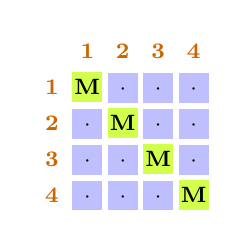
\begin{tikzpicture}
    \matrix[matrix of nodes,
            nodes in empty cells,
            ampersand replacement=\&,
            nodes={minimum size=0.38cm, text width=0.38cm, inner sep=0pt, align=center, font=\footnotesize, execute at begin node={\vphantom{0}}},
            row sep=2pt,
            column sep=2pt] {
      {} \& |[font=\footnotesize\bfseries, text=orange!80!black]| 1 \& |[font=\footnotesize\bfseries, text=orange!80!black]| 2 \& |[font=\footnotesize\bfseries, text=orange!80!black]| 3 \& |[font=\footnotesize\bfseries, text=orange!80!black]| 4 \\
      |[font=\footnotesize\bfseries, text=orange!80!black]| 1 \& |[fill=lime!70]| \textbf{M} \& |[fill=blue!25]| $\cdot$ \& |[fill=blue!25]| $\cdot$ \& |[fill=blue!25]| $\cdot$ \\
      |[font=\footnotesize\bfseries, text=orange!80!black]| 2 \& |[fill=blue!25]| $\cdot$ \& |[fill=lime!70]| \textbf{M} \& |[fill=blue!25]| $\cdot$ \& |[fill=blue!25]| $\cdot$ \\
      |[font=\footnotesize\bfseries, text=orange!80!black]| 3 \& |[fill=blue!25]| $\cdot$ \& |[fill=blue!25]| $\cdot$ \& |[fill=lime!70]| \textbf{M} \& |[fill=blue!25]| $\cdot$ \\
      |[font=\footnotesize\bfseries, text=orange!80!black]| 4 \& |[fill=blue!25]| $\cdot$ \& |[fill=blue!25]| $\cdot$ \& |[fill=blue!25]| $\cdot$ \& |[fill=lime!70]| \textbf{M} \\
    };
    \end{tikzpicture}
    \end{center}

    \column{0.5\textwidth}
    \begin{block}{Diagonala secundară}
      De la \texttt{(1,n)} la \texttt{(n,1)}.\\
      Condiție: $i + j = n + 1$
    \end{block}
    \begin{center}
    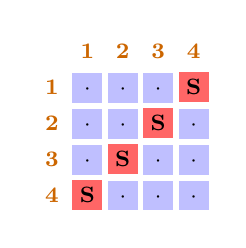
\begin{tikzpicture}
    \matrix[matrix of nodes,
            nodes in empty cells,
            ampersand replacement=\&,
            nodes={minimum size=0.38cm, text width=0.38cm, inner sep=0pt, align=center, font=\footnotesize, execute at begin node={\vphantom{0}}},
            row sep=2pt,
            column sep=2pt] {
      {} \& |[font=\footnotesize\bfseries, text=orange!80!black]| 1 \& |[font=\footnotesize\bfseries, text=orange!80!black]| 2 \& |[font=\footnotesize\bfseries, text=orange!80!black]| 3 \& |[font=\footnotesize\bfseries, text=orange!80!black]| 4 \\
      |[font=\footnotesize\bfseries, text=orange!80!black]| 1 \& |[fill=blue!25]| $\cdot$ \& |[fill=blue!25]| $\cdot$ \& |[fill=blue!25]| $\cdot$ \& |[fill=red!60]| \textbf{S} \\
      |[font=\footnotesize\bfseries, text=orange!80!black]| 2 \& |[fill=blue!25]| $\cdot$ \& |[fill=blue!25]| $\cdot$ \& |[fill=red!60]| \textbf{S} \& |[fill=blue!25]| $\cdot$ \\
      |[font=\footnotesize\bfseries, text=orange!80!black]| 3 \& |[fill=blue!25]| $\cdot$ \& |[fill=red!60]| \textbf{S} \& |[fill=blue!25]| $\cdot$ \& |[fill=blue!25]| $\cdot$ \\
      |[font=\footnotesize\bfseries, text=orange!80!black]| 4 \& |[fill=red!60]| \textbf{S} \& |[fill=blue!25]| $\cdot$ \& |[fill=blue!25]| $\cdot$ \& |[fill=blue!25]| $\cdot$ \\
    };
    \end{tikzpicture}
    \end{center}
  \end{columns}

  \smallskip
  Dacă $n$ este impar, cele două diagonale au un element comun (centrul matricei).
\end{frame}

\begin{frame}[fragile]{Parcurgerea diagonalelor}
  \begin{lstlisting}
// diagonala principala: conditia i == j
for (int i = 1; i <= n; i++)
    // a[i][i]

// diagonala secundara: conditia i + j == n + 1
for (int i = 1; i <= n; i++)
    // a[i][n + 1 - i]
  \end{lstlisting}

  \begin{itemize}
    \item Ambele diagonale au $n$ elemente $\rightarrow$ complexitate $O(n)$
    \item \textbf{Atenție:} la indexare de la 0 condiția diagonalei secundare devine $i + j = n - 1$, nu $n + 1$
  \end{itemize}
\end{frame}

% ================================================================
\section{Împărțirea în zone}

\begin{frame}{Zone față de diagonala principală}
  \begin{columns}[T]
    \column{0.48\textwidth}
    \begin{center}
    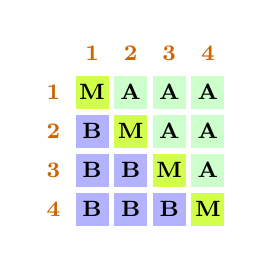
\begin{tikzpicture}
    \matrix[matrix of nodes,
            nodes in empty cells,
            ampersand replacement=\&,
            nodes={minimum size=0.42cm, text width=0.42cm, inner sep=0pt, align=center, font=\footnotesize, execute at begin node={\vphantom{0}}},
            row sep=2pt,
            column sep=2pt] {
      {} \& |[font=\footnotesize\bfseries, text=orange!80!black]| 1 \& |[font=\footnotesize\bfseries, text=orange!80!black]| 2 \& |[font=\footnotesize\bfseries, text=orange!80!black]| 3 \& |[font=\footnotesize\bfseries, text=orange!80!black]| 4 \\
      |[font=\footnotesize\bfseries, text=orange!80!black]| 1 \& |[fill=lime!70]| \textbf{M} \& |[fill=green!20]| \textbf{A} \& |[fill=green!20]| \textbf{A} \& |[fill=green!20]| \textbf{A} \\
      |[font=\footnotesize\bfseries, text=orange!80!black]| 2 \& |[fill=blue!30]| \textbf{B} \& |[fill=lime!70]| \textbf{M} \& |[fill=green!20]| \textbf{A} \& |[fill=green!20]| \textbf{A} \\
      |[font=\footnotesize\bfseries, text=orange!80!black]| 3 \& |[fill=blue!30]| \textbf{B} \& |[fill=blue!30]| \textbf{B} \& |[fill=lime!70]| \textbf{M} \& |[fill=green!20]| \textbf{A} \\
      |[font=\footnotesize\bfseries, text=orange!80!black]| 4 \& |[fill=blue!30]| \textbf{B} \& |[fill=blue!30]| \textbf{B} \& |[fill=blue!30]| \textbf{B} \& |[fill=lime!70]| \textbf{M} \\
    };
    \end{tikzpicture}
    \end{center}

    \column{0.52\textwidth}
    \begin{itemize}
      \item \colorbox{lime!70}{\textbf{M}} $i = j$: pe diagonală
      \item \colorbox{green!20}{\textbf{A}} $i < j$: deasupra diagonalei
      \item \colorbox{blue!30}{\textbf{B}} $i > j$: sub diagonală
    \end{itemize}

    \smallskip
    Condiția depinde \textbf{doar de indici}, nu de valorile elementelor.
  \end{columns}
\end{frame}

\begin{frame}{Zone față de diagonala secundară}
  Pentru $n = 4$ ($n + 1 = 5$):

  \begin{columns}[T]
    \column{0.48\textwidth}
    \begin{center}
    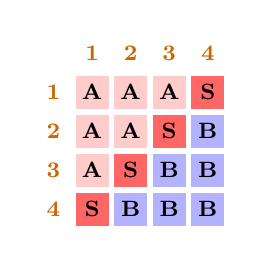
\begin{tikzpicture}
    \matrix[matrix of nodes,
            nodes in empty cells,
            ampersand replacement=\&,
            nodes={minimum size=0.42cm, text width=0.42cm, inner sep=0pt, align=center, font=\footnotesize, execute at begin node={\vphantom{0}}},
            row sep=2pt,
            column sep=2pt] {
      {} \& |[font=\footnotesize\bfseries, text=orange!80!black]| 1 \& |[font=\footnotesize\bfseries, text=orange!80!black]| 2 \& |[font=\footnotesize\bfseries, text=orange!80!black]| 3 \& |[font=\footnotesize\bfseries, text=orange!80!black]| 4 \\
      |[font=\footnotesize\bfseries, text=orange!80!black]| 1 \& |[fill=red!20]| \textbf{A} \& |[fill=red!20]| \textbf{A} \& |[fill=red!20]| \textbf{A} \& |[fill=red!60]| \textbf{S} \\
      |[font=\footnotesize\bfseries, text=orange!80!black]| 2 \& |[fill=red!20]| \textbf{A} \& |[fill=red!20]| \textbf{A} \& |[fill=red!60]| \textbf{S} \& |[fill=blue!30]| \textbf{B} \\
      |[font=\footnotesize\bfseries, text=orange!80!black]| 3 \& |[fill=red!20]| \textbf{A} \& |[fill=red!60]| \textbf{S} \& |[fill=blue!30]| \textbf{B} \& |[fill=blue!30]| \textbf{B} \\
      |[font=\footnotesize\bfseries, text=orange!80!black]| 4 \& |[fill=red!60]| \textbf{S} \& |[fill=blue!30]| \textbf{B} \& |[fill=blue!30]| \textbf{B} \& |[fill=blue!30]| \textbf{B} \\
    };
    \end{tikzpicture}
    \end{center}

    \column{0.52\textwidth}
    \begin{itemize}
      \item \colorbox{red!60}{\textbf{S}} $i + j = n + 1$: pe diagonală
      \item \colorbox{red!20}{\textbf{A}} $i + j < n + 1$: deasupra
      \item \colorbox{blue!30}{\textbf{B}} $i + j > n + 1$: sub diagonală
    \end{itemize}

    \smallskip
    \textbf{Atenție:} la indexare de la 0, pragul este $n - 1$, nu $n + 1$.
  \end{columns}
\end{frame}

\begin{frame}[fragile]{Exemplu: suma elementelor din fiecare zonă}
  \begin{lstlisting}
long long sp = 0; // suma deasupra diag. principale
long long sd = 0; // suma sub diagonala principala

for (int i = 1; i <= n; i++)
    for (int j = 1; j <= n; j++) {
        if (i < j) sp += a[i][j];
        if (i > j) sd += a[i][j];
    }
  \end{lstlisting}

  \begin{itemize}
    \item Parcurgem matricea o singură dată: $O(n^2)$
    \item Putem combina condițiile pentru mai multe zone în aceeași buclă
    \item \textbf{Optimizare:} calculăm sumele \emph{în timp ce citim} \textemdash{} nu e nevoie să stocăm matricea
  \end{itemize}
\end{frame}

% ================================================================
\section{Transformări}

\begin{frame}[fragile]{Transpusa matricei}
  \textbf{Transpusa} reflectă matricea față de diagonala principală: $b[j][i] = a[i][j]$.

  \begin{lstlisting}
// transpusa intr-o matrice auxiliara
int b[NMAX][NMAX];
for (int i = 1; i <= n; i++)
    for (int j = 1; j <= m; j++)
        b[j][i] = a[i][j];
// b are m linii si n coloane
  \end{lstlisting}

  \smallskip
  Pentru matrice \textbf{pătratică}, transpusa se poate face în loc (\emph{in-place}):
  \begin{lstlisting}
for (int i = 1; i <= n; i++)
    for (int j = i + 1; j <= n; j++)
        swap(a[i][j], a[j][i]);
  \end{lstlisting}
\end{frame}

\begin{frame}[fragile]{Oglindire}
  \begin{columns}[T]
    \column{0.5\textwidth}
    \textbf{Vertical} (inversăm liniile):
    \begin{lstlisting}
for (int i = 1; i <= n / 2; i++)
  for (int j = 1; j <= m; j++)
    swap(a[i][j],
         a[n + 1 - i][j]);
    \end{lstlisting}

    \column{0.5\textwidth}
    \textbf{Orizontal} (inversăm coloanele):
    \begin{lstlisting}
for (int i = 1; i <= n; i++)
  for (int j = 1; j <= m / 2; j++)
    swap(a[i][j],
         a[i][m + 1 - j]);
    \end{lstlisting}
  \end{columns}

  \smallskip
  \begin{itemize}
    \item Complexitate: $O(n \cdot m)$ pentru fiecare operație
    \item \textbf{Rotire 90°} la dreapta $=$ transpusă $+$ oglindire orizontală
  \end{itemize}
\end{frame}

% ================================================================
\section{Recapitulare}

\begin{frame}{Recapitulare}
  Orice algoritm care parcurge \textbf{toată} matricea (parcurgere, sume pe zone, transpusă, oglindire etc.) are complexitate:

  \begin{center}
  \begin{tabular}{ll}
    \toprule
    Matrice & Complexitate \\
    \midrule
    $n \times m$ (dreptunghiulară) & $O(n \cdot m)$ \\
    $n \times n$ (pătratică)       & $O(n^2)$       \\
    \bottomrule
  \end{tabular}
  \end{center}

  \smallskip
  Excepții (parcurgere parțială):
  \begin{itemize}
    \item O linie sau coloană: $O(m)$ respectiv $O(n)$
    \item O diagonală: $O(n)$
  \end{itemize}
\end{frame}

% ================================================================
\section{Resurse}

\begin{frame}{Resurse}
  \begin{itemize}\itemsep6pt
    \item \href{https://www.pbinfo.ro/articole/5620/tablouri-bidimensionale}{\textbf{pbinfo.ro}} \textemdash{} Tablouri bidimensionale
    \item \href{https://www.pbinfo.ro/articole/5622/declararea-matricelor-referirea-elementelor}{\textbf{pbinfo.ro}} \textemdash{} Declararea matricelor. Referirea elementelor
    \item \href{https://www.pbinfo.ro/articole/5623/parcurgerea-tablourilor-bidimensionale}{\textbf{pbinfo.ro}} \textemdash{} Parcurgerea tablourilor bidimensionale
    \item \href{https://www.pbinfo.ro/articole/5626/tablouri-patratice}{\textbf{pbinfo.ro}} \textemdash{} Tablouri pătratice
  \end{itemize}
\end{frame}

% ================================================================
\section{Probleme de antrenament}

\begin{frame}{Probleme de antrenament}
  \begin{block}{Parcurgerea matricilor oarecare}
    \begin{itemize}\footnotesize\itemsep0pt
      \item \href{https://code.algolymp.com/problems/996}{\textbf{Sum Even \#996}} {\footnotesize\textcolor{gray}{(AlgoCode)}}
      \item \href{https://code.algolymp.com/problems/988}{\textbf{Algorithm Task \#988}} {\footnotesize\textcolor{gray}{(AlgoCode)}}
      \item \href{https://code.algolymp.com/problems/1625}{\textbf{Algorithm Task \#1625}} {\footnotesize\textcolor{gray}{(AlgoCode)}}
    \end{itemize}
  \end{block}
  \vspace{-4pt}
  \begin{block}{Parcurgerea matricilor pătratice}
    \begin{itemize}\footnotesize\itemsep0pt
      \item \href{https://code.algolymp.com/problems/1006}{\textbf{Algorithm Task \#1006}} {\footnotesize\textcolor{gray}{(AlgoCode)}}
      \item \href{https://code.algolymp.com/problems/1004}{\textbf{Algorithm Task \#1004}} {\footnotesize\textcolor{gray}{(AlgoCode)}}
      \item \href{https://code.algolymp.com/problems/999}{\textbf{Algorithm Task \#999}} {\footnotesize\textcolor{gray}{(AlgoCode)}}
    \end{itemize}
  \end{block}
  \vspace{-4pt}
  \begin{block}{Generarea matricilor}
    \begin{itemize}\footnotesize\itemsep0pt
      \item \href{https://code.algolymp.com/problems/963}{\textbf{Sequence Mat \#963}} {\footnotesize\textcolor{gray}{(AlgoCode)}}
      \item \href{https://code.algolymp.com/problems/968}{\textbf{Sequence Mat \#968}} {\footnotesize\textcolor{gray}{(AlgoCode)}}
      \item \href{https://code.algolymp.com/problems/973}{\textbf{Sequence Mat 17 \#973}} {\footnotesize\textcolor{gray}{(AlgoCode)}}
    \end{itemize}
  \end{block}
\end{frame}

\end{document}
